\documentclass{article}

% =========================================================
% CONFIGURACIÓN GENERAL Y MÁRGENES
% =========================================================

\usepackage[
    letterpaper,
    top=2cm,
    bottom=3cm,
    left=3cm,
    right=3cm,
    marginparwidth=1.75cm
]{geometry}

\usepackage[spanish, es-tabla]{babel}
\usepackage[utf8]{inputenc}
\usepackage[T1]{fontenc}

% =========================================================
% PAQUETES MATEMÁTICOS Y GRÁFICOS
% =========================================================

\usepackage{amsmath}
\usepackage{amssymb}
\usepackage{graphicx}
\usepackage{fancyhdr}
\usepackage{tabularx}
\usepackage{booktabs}
\usepackage{float}
\usepackage{caption}
\usepackage{xcolor}
\usepackage{listings}

% =========================================================
% CONFIGURACIÓN DE LISTINGS (CÓDIGO PYTHON)
% =========================================================

\definecolor{codegreen}{rgb}{0,0.6,0}
\definecolor{codegray}{rgb}{0.5,0.5,0.5}
\definecolor{codepurple}{rgb}{0.58,0,0.82}
\definecolor{backcolour}{rgb}{0.96,0.96,0.96}

\lstdefinestyle{mystyle}{
    backgroundcolor=\color{backcolour},   
    commentstyle=\color{codegreen},
    keywordstyle=\color{magenta},
    numberstyle=\tiny\color{codegray},
    stringstyle=\color{codepurple},
    basicstyle=\ttfamily\footnotesize,
    breakatwhitespace=false,         
    breaklines=true,                 
    captionpos=b,                    
    keepspaces=true,                 
    numbers=left,                    
    numbersep=5pt,                  
    showspaces=false,                
    showstringspaces=false,
    showtabs=false,                  
    tabsize=4
}
\lstset{style=mystyle}

% =========================================================
% REFERENCIAS BIBLIOGRÁFICAS (BIBLATEX - IEEE)
% =========================================================

\usepackage[
    backend=biber,
    style=ieee,
    sorting=none
]{biblatex}

\addbibresource{referencias.bib}

% =========================================================
% HIPERVÍNCULOS
% =========================================================

\usepackage[
    colorlinks=true,
    allcolors=blue
]{hyperref}

% =========================================================
% ENCABEZADO Y PIE DE PÁGINA INSTITUCIONAL (UTA - FISEI)
% =========================================================

\pagestyle{fancy}
\fancyhf{}

\setlength{\headheight}{70pt}

\fancyhead[C]{%
    \begin{minipage}[c]{2.5cm}
        \centering
        
\includegraphics[width=2.2cm]{imagenes/uta.png}
    \end{minipage}%
    \hfill
    \begin{minipage}[c]{8cm}
        \centering
        \small{\textbf{UNIVERSIDAD TÉCNICA DE AMBATO}}\\[0.1cm]
        \scriptsize{\textit{FACULTAD DE INGENIERÍA EN SISTEMAS, ELECTRÓNICA E INDUSTRIAL}}\\[0.1cm]
        \scriptsize{\textbf{CARRERA DE SOFTWARE}}\\[0.1cm]
        \scriptsize{\textbf{CICLO ACADÉMICO: OCTUBRE 2026 -- MARZO 2027}}
    \end{minipage}%
    \hfill
    \begin{minipage}[c]{2.5cm}
        \centering
        
\includegraphics[width=2.2cm]{imagenes/fisei.png}
    \end{minipage}%
}

\fancyfoot[C]{\thepage}

% =========================================================
% DOCUMENTO PRINCIPAL
% =========================================================

\begin{document}

% =========================================================
% PORTADA
% =========================================================

\begin{titlepage}

    \thispagestyle{empty}

    \begin{center}

        \vspace*{0.5cm}

        
\includegraphics[width=4cm]{imagenes/uta.png}

        \vspace{0.7cm}

        {\Large \textbf{UNIVERSIDAD TÉCNICA DE AMBATO}}

        \vspace{0.35cm}

        {\large
        FACULTAD DE INGENIERÍA EN SISTEMAS,\\
        ELECTRÓNICA E INDUSTRIAL}

        \vspace{0.35cm}

        {\large \textbf{CARRERA DE SOFTWARE}}

        {\large
        \vspace{1.5cm}
        \textbf{Tema:}\\
        REDUCCIÓN MATRICIAL DE IMÁGENES MEDIANTE MUESTREO ESPACIAL, APROVECHAMIENTO DE REDUNDANCIA Y FILTRADO DISCRETO SIN FUNCIONES DE LIBRERÍA

        \vspace{0.45cm}

        \textbf{Unidad de Organización Curricular:}\\
        Profesional

        \vspace{0.45cm}

        \textbf{Nivel y Paralelo:}\\
        7mo -- A

        \vspace{0.45cm}

        \textbf{Asignatura:}\\
        Inteligencia Artificial

        \vspace{0.45cm}

        \textbf{Docente:}\\
        Ing. Mg. Ruben Nogales

        \vspace{0.45cm}

        \textbf{Alumnos participantes:}\\
        Toala Steeven\\
        Chavez Michael

        }

        \vfill

        {\large
        Ambato -- Ecuador\\
        Octubre de 2026
        }

    \end{center}

\end{titlepage}

% =========================================================
% ÍNDICES (ROMANOS)
% =========================================================

\pagenumbering{roman}

\tableofcontents
\newpage

\listoffigures
\listoftables
\newpage

\pagenumbering{arabic}

% =========================================================
% 1. INTRODUCCIÓN Y PLANTEAMIENTO DEL PROBLEMA
% =========================================================

\section{Introducción y Planteamiento del Problema}

En el ámbito del \textbf{Procesamiento Digital de Imágenes} y la \textbf{Inteligencia Artificial}, las imágenes capturadas por sensores ópticos representan volúmenes masivos de datos digitales. En aplicaciones prácticas como la visión artificial por computador, el reconocimiento biométrico, la robótica móvil y el entrenamiento de modelos de aprendizaje profundo (\textit{Deep Learning} mediante Redes Neuronales Convolucionales o CNNs), el procesamiento directo de imágenes en alta resolución impone una carga computacional prohibitiva en términos de memoria RAM, ancho de banda y tiempo de cómputo \cite{szeliski2022computer}.

Frente a esta problemática, la reducción dimensional o cambio de escala espacial (\textit{downsampling}) constituye una de las etapas esenciales de acondicionamiento de datos. No obstante, en la práctica académica y profesional contemporánea es común el empleo indiscriminado de funciones de caja negra provenientes de librerías comerciales o de código abierto, tales como \texttt{cv2.resize} en OpenCV \cite{bradski2000opencv} o \texttt{imresize} en MATLAB. Dichas funciones aplican de manera opaca algoritmos complejos de interpolación bilineal, bicúbica, \textit{splines} o filtros Lanczos, ocultando los principios matemáticos fundacionales de la teoría de señales: el \textbf{muestreo espacial discreto}, la manipulación de índices en matrices bidimensionales y el aprovechamiento de la \textbf{redundancia espacial de píxeles} \cite{gonzalez2018digital}.

Por tal motivo, el presente proyecto se desarrolla bajo la restricción pedagógica explícita de \textbf{prohibición total de funciones automáticas de cambio de escala}. En su lugar, se implementan desde cero, mediante programación matricial pura en Python y NumPy \cite{harris2020array}, cuatro métodos de reducción dimensional sobre matrices impares ($3\times3, 5\times5, 7\times7$):
\begin{enumerate}
    \item \textbf{Submuestreo por Decimación Espacial (Saltos):} Muestreo periódico de la matriz omitiendo píxeles intermedios.
    \item \textbf{Promedio de Bloques Redundantes (\textit{Mean Pooling}):} Integración de la luminosidad de píxeles vecinos mediante la media aritmética.
    \item \textbf{Filtro Mediana de Bloques (\textit{Median Pooling}):} Selección del elemento central ordenado con alta inmunidad a ruido impulsivo.
    \item \textbf{Ponderación Gaussiana Bidimensional Discreta:} Convolución local mediante una máscara normalizada con decaimiento radial.
\end{enumerate}

Los objetivos planteados para la práctica son:
\begin{itemize}
    \item Implementar de forma manual y vectorizada los cuatro algoritmos de reducción en Python sin utilizar comandos empaquetados de redimensionamiento.
    \item Demostrar analítica y visualmente por qué las imágenes reducidas conservan su inteligibilidad geométrica gracias a la redundancia espacial.
    \item Justificar rigurosamente la necesidad matemática del empleo de matrices y saltos de orden impar ($3\times3, 5\times5, 7\times7$).
    \item Evaluar cuantitativamente la compresión de datos y la tasa de ahorro espacial obtenida para distintos factores de paso $k$.
\end{itemize}

% =========================================================
% 2. MARCO TEÓRICO Y FORMULACIÓN MATEMÁTICA
% =========================================================

\section{Marco Teórico y Formulación Matemática}

\subsection{Representación Matricial de la Imagen Digital}
Una imagen digital monocromática continua se modela matemáticamente como una función bidimensional de intensidad lumínica $f(x, y)$. En el dominio discreto computacional, tras los procesos físicos de muestreo espacial y cuantización radiométrica, la imagen se representa como una matriz numérica bidimensional $I \in \mathbb{R}^{M \times N}$:
\begin{equation}
    I = \begin{bmatrix}
        I(0, 0) & I(0, 1) & \cdots & I(0, N-1) \\
        I(1, 0) & I(1, 1) & \cdots & I(1, N-1) \\
        \vdots & \vdots & \ddots & \vdots \\
        I(M-1, 0) & I(M-1, 1) & \cdots & I(M-1, N-1)
    \end{bmatrix}
\end{equation}
donde cada elemento $I(i, j)$ representa un \textbf{píxel} cuya intensidad para una resolución radiométrica estándar de 8 bits está acotada en el intervalo cerrado de enteros:
\begin{equation}
    I(i, j) \in \{0, 1, 2, \dots, 255\} \subset \mathbb{Z}
\end{equation}
donde $0$ denota la ausencia total de luz (negro puro) y $255$ representa la saturación máxima (blanco puro). Para imágenes a color en el espacio RGB, la representación se extiende a un tensor tridimensional de orden $M \times N \times 3$, compuesto por tres matrices desacopladas correspondientes a los canales Rojo ($R$), Verde ($G$) y Azul ($B$) \cite{jain1989fundamentals}.

\subsection{El Principio de Redundancia Espacial}
En escenas del mundo físico real, los objetos presentan coherencia geométrica y superficies continuas (paredes, rostros, cielo, vestimenta). Como consecuencia física directa, dos píxeles contiguos en coordenadas $(i, j)$ y $(i, j+1)$ exhiben una correlación estadística sumamente alta:
\begin{equation}
    |I(i, j) - I(i, j+1)| \approx 0
\end{equation}
Esta propiedad se denomina \textbf{redundancia espacial}. Significa que gran parte de los píxeles adyacentes no aportan información estructural nueva, sino que replican la luminosidad de su entorno. Por ende, al reducir las dimensiones espaciales mediante muestreo o promediado, la estructura global, bordes y formas macroscópicas permanecen plenamente discernibles para el sistema visual humano.

\subsection{Método 1: Submuestreo por Saltos (Decimación Espacial)}
El método más elemental de reducción consiste en recorrer la matriz original dando saltos de tamaño fijo $k \in \mathbb{N}$ tanto en las filas como en las columnas. Si la matriz original posee dimensiones $M \times N$, la nueva matriz reducida $I_{\text{saltos}}$ tendrá dimensiones:
\begin{equation}
    M' = \left\lfloor \frac{M}{k} \right\rfloor, \quad N' = \left\lfloor \frac{N}{k} \right\rfloor
\end{equation}
La correspondencia determinística entre las coordenadas del píxel reducido $(i, j)$ y el píxel original viene dada por:
\begin{equation}
    \label{eq:saltos}
    I_{\text{saltos}}(i, j) = I_{\text{original}}(i \cdot k, j \cdot k)
\end{equation}
\textbf{Análisis de Señal y Aliasing:} De acuerdo con el Teorema de Muestreo de Nyquist-Shannon \cite{shannon1949communication}, para reconstruir o representar fidedignamente una señal continua, la frecuencia de muestreo espacial $f_s$ debe ser al menos el doble de la frecuencia espacial máxima presente en la imagen ($f_s \ge 2 f_{\max}$). Al aplicar decimación directa sin filtrado previo, las frecuencias espaciales altas que superen el límite de Nyquist se solapan sobre las bajas frecuencias, provocando artefactos de \textbf{aliasing} o escalonamiento visible (bordes dentados y patrones de Moiré).

\subsection{Método 2: Promedio de Bloques Redundantes (Mean Pooling)}
Para mitigar el descarte destructivo de información del submuestreo directo, el método de promedio integra la información de todos los $k \times k$ píxeles que conforman la vecindad o bloque local. Cada celda de la imagen reducida se calcula como la media aritmética de su bloque asociado:
\begin{equation}
    \label{eq:promedio}
    I_{\text{promedio}}(i, j) = \text{redondear}\left( \frac{1}{k^2} \sum_{u=0}^{k-1} \sum_{v=0}^{k-1} I_{\text{original}}(i \cdot k + u, j \cdot k + v) \right)
\end{equation}
\textbf{Ventaja Física:} Este método equivale a aplicar un filtro de caja (\textit{Box Filter}) de paso bajo antes de la decimación. Al promediar los $k^2$ píxeles redundantes, se suavizan las altas frecuencias espaciales, preservando la energía lumínica total de la escena y atenuando significativamente el efecto de aliasing en los bordes.

\subsection{Método 3: Reducción por Filtro Mediana (Median Pooling)}
El filtro mediana es un operador no lineal de vecindad. En lugar de computar una combinación lineal ponderada, extrae el conjunto de los $k^2$ valores discretos del bloque:
\begin{equation}
    \mathcal{B}_{i, j} = \{ I_{\text{original}}(i \cdot k + u, j \cdot k + v) \mid 0 \le u < k, \; 0 \le v < k \}
\end{equation}
Dichos valores se ordenan de menor a mayor en una secuencia monotónica $\{v_{(1)}, v_{(2)}, \dots, v_{(k^2)}\}$. La intensidad del píxel resultante corresponde al valor ubicado en la posición central:
\begin{equation}
    \label{eq:mediana}
    I_{\text{mediana}}(i, j) = v_{\left( \frac{k^2 + 1}{2} \right)}
\end{equation}
\textbf{Propiedad Antirruido:} A diferencia del promedio aritmético, que es sumamente vulnerable a valores atípicos (\textit{outliers}), la mediana es altamente robusta frente a ruido impulsivo (sal y pimienta), preservando discontinuidades y bordes afilados sin generar halos difusos.

\subsection{Método 4: Filtrado Gaussiano Ponderado 2D}
La convolución gaussiana asigna coeficientes de ponderación espacialmente simétricos, donde los píxeles cercanos al centro geométrico del bloque reciben mayor peso que los de la periferia, imitando la función de dispersión de punto (\textit{Point Spread Function}) del sistema visual humano. La función gaussiana continua bidimensional isotrópica con media cero y desviación estándar $\sigma$ se define como:
\begin{equation}
    G(x, y) = \frac{1}{2\pi \sigma^2} \exp\left( -\frac{x^2 + y^2}{2\sigma^2} \right)
\end{equation}
En el espacio discreto para una matriz de tamaño $k \times k$, las coordenadas espaciales se centran en el origen mediante:
\begin{equation}
    x, y \in \left\{ -\frac{k-1}{2}, \dots, 0, \dots, \frac{k-1}{2} \right\}, \quad \sigma = \frac{k}{3}
\end{equation}
Para garantizar que la transformación no altere la ganancia lumínica global de la imagen, la matriz de coeficientes $K(u, v)$ se normaliza estrictamente de forma que la suma de todos sus elementos sea idénticamente $1.0$:
\begin{equation}
    K(u, v) = \frac{G(u, v)}{\sum_{p} \sum_{q} G(p, q)}, \quad \text{tal que} \quad \sum_{u=0}^{k-1} \sum_{v=0}^{k-1} K(u, v) = 1.0
\end{equation}
El valor del píxel reducido se obtiene mediante la suma de productos discretos:
\begin{equation}
    \label{eq:gauss}
    I_{\text{gauss}}(i, j) = \text{redondear}\left( \sum_{u=0}^{k-1} \sum_{v=0}^{k-1} I_{\text{original}}(i \cdot k + u, j \cdot k + v) \cdot K(u, v) \right)
\end{equation}

\subsection{Fundamentación del Uso Estricto de Matrices Impares \texorpdfstring{($3\times3, 5\times5, 7\times7$)}{(3x3, 5x5, 7x7)}}
La selección obligatoria de factores de salto y matrices de orden impar obedece a tres principios matemáticos fundamentales de la visión artificial:
\begin{enumerate}
    \item \textbf{Existencia de un Centro Geométrico Entero Simétrico:} Una matriz de orden impar $k \times k$ posee un único centro geométrico situado exactamente en las coordenadas enteras:
    \begin{equation}
        (c_x, c_y) = \left( \frac{k-1}{2}, \frac{k-1}{2} \right) \in \mathbb{N}^2
    \end{equation}
    Por el contrario, en matrices pares ($2\times2, 4\times4$), el centro teórico cae en coordenadas fraccionarias ($0.5, 1.5$), careciendo de un píxel físico sobre el cual anclar simétricamente la operación.
    \item \textbf{Cálculo de Mediana Pura sin Aproximaciones:} Para un bloque impar, el cardinal del conjunto es $k^2 \in \{9, 25, 49\}$, el cual es siempre un número impar. En consecuencia, la mediana corresponde de forma exacta y pura a un valor real existente dentro de la muestra:
    \begin{equation}
        \text{Posición central exacta} = \frac{k^2 + 1}{2} \in \mathbb{Z}
    \end{equation}
    En bloques pares ($k^2 = 4, 16, 64$), la mediana requeriría promediar los dos elementos centrales, desvirtuando la naturaleza no lineal del filtro.
    \item \textbf{Isotropía y Simetría Radial Gaussiana:} La campana de Gauss requiere distribuirse simétricamente alrededor de un pico central máximo en $(0, 0)$. Solo las matrices impares permiten ubicar el vértice de la campana en el píxel central y distribuir los pesos equitativamente en los cuatro cuadrantes espaciales.
\end{enumerate}

% =========================================================
% 3. CORRESPONDENCIA ENTRE NOTACIÓN Y VARIABLES EN PYTHON
% =========================================================

\section{Correspondencia entre Notación Matemática y Variables del Software}

Con el fin de garantizar máxima transparencia y trazabilidad entre la fundamentación matemática y el código implementado, la Tabla~\ref{tab:equivalencias} detalla la correspondencia unívoca entre los símbolos de las ecuaciones y las variables definidas en Python.

\begin{table}[H]
    \centering
    \caption{Correspondencia entre la notación matemática teórica y las variables del software}
    \label{tab:equivalencias}
    \small
    \begin{tabularx}{\textwidth}{l >{\raggedright\arraybackslash}p{6.2cm} >{\raggedright\arraybackslash}X}
        \toprule
        \textbf{Símbolo} & \textbf{Significado Conceptual} & \textbf{Variable en Python (\texttt{main.py})} \\
        \midrule
        $M \times N$ & Dimensiones originales de la imagen (alto $\times$ ancho) & \texttt{alto\_orig}, \texttt{ancho\_orig} \\
        $k \in \{3, 5, 7\}$ & Factor de salto impar del bloque espacial & \texttt{paso\_k} \\
        $M' \times N'$ & Dimensiones de la imagen reducida & \texttt{alto\_nuevo}, \texttt{ancho\_nuevo} \\
        $k^2$ & Cantidad total de píxeles por bloque ($9, 25, 49$) & \texttt{total\_pixeles\_bloque} \\
        $I_{\text{original}}(i\cdot k, j\cdot k)$ & Píxel discreto muestreado por saltos & \texttt{imagen\_reducida[fila, col]} \\
        $\frac{1}{k^2} \sum I$ & Media aritmética del bloque redundante & \texttt{promedio} \\
        $v_{\left(\frac{k^2+1}{2}\right)}$ & Mediana del bloque ordenado & \texttt{mediana\_valor} \\
        $K(u, v)$ & Kernel gaussiano bidimensional normalizado & \texttt{kernel\_normalizado} \\
        $\sigma = k/3$ & Desviación estándar de la máscara gaussiana & \texttt{desviacion\_estandar} \\
        $1 - \frac{M'N'}{MN}$ & Porcentaje de reducción de datos y memoria & \texttt{porcentaje\_ahorro} \\
        \bottomrule
    \end{tabularx}
\end{table}

% =========================================================
% 4. IMPLEMENTACIÓN DEL ALGORITMO EN PYTHON
% =========================================================

\section{Implementación del Algoritmo en Python}

El sistema fue desarrollado en el lenguaje de programación Python utilizando operaciones matriciales directas con la biblioteca \texttt{NumPy} \cite{harris2020array} y visualización científica con \texttt{Matplotlib} \cite{hunter2007matplotlib}. Se evitó rigurosamente cualquier llamada a funciones cerradas como \texttt{cv2.resize}.

\subsection{Código Fuente de los Algoritmos de Reducción}
A continuación se presentan los fragmentos de código modular correspondientes a los cuatro métodos implementados en el archivo \texttt{codigo/main.py}:

\begin{lstlisting}[language=Python, caption={Implementación de los algoritmos de reducción matricial sin funciones de librería}]
import numpy as np

def generar_kernel_gaussiano(paso_k: int) -> np.ndarray:
    """Genera kernel gaussiano 2D normalizado (suma total = 1.0)."""
    desviacion_estandar = paso_k / 3.0
    rango_ejes = np.linspace(-(paso_k - 1) / 2.0, (paso_k - 1) / 2.0, paso_k)
    curva_gaussiana = np.exp(-0.5 * np.square(rango_ejes) / np.square(desviacion_estandar))
    kernel_2d = np.outer(curva_gaussiana, curva_gaussiana)
    return kernel_2d / np.sum(kernel_2d)

def reducir_por_saltos(imagen_original: np.ndarray, paso_k: int) -> np.ndarray:
    """Muestreo espacial directo dando saltos de 'paso_k' pixeles."""
    alto_n = imagen_original.shape[0] // paso_k
    ancho_n = imagen_original.shape[1] // paso_k
    canales = imagen_original.shape[2] if imagen_original.ndim == 3 else 1
    
    # Decimacion espacial directa mediante saltos matriciales
    if imagen_original.ndim == 2:
        return imagen_original[::paso_k, ::paso_k][:alto_n, :ancho_n].copy()
    else:
        return imagen_original[::paso_k, ::paso_k, :][:alto_n, :ancho_n, :].copy()

def reducir_por_promedio(imagen_original: np.ndarray, paso_k: int) -> np.ndarray:
    """Aprovechamiento de redundancia mediante media aritmetica (Mean Pooling)."""
    alto_n = imagen_original.shape[0] // paso_k
    ancho_n = imagen_original.shape[1] // paso_k
    recorte = imagen_original[:alto_n * paso_k, :ancho_n * paso_k]
    
    if imagen_original.ndim == 2:
        bloques = recorte.reshape(alto_n, paso_k, ancho_n, paso_k)
        return np.round(bloques.mean(axis=(1, 3))).astype(np.uint8)
    else:
        canales = imagen_original.shape[2]
        bloques = recorte.reshape(alto_n, paso_k, ancho_n, paso_k, canales)
        return np.round(bloques.mean(axis=(1, 3))).astype(np.uint8)

def reducir_por_mediana(imagen_original: np.ndarray, paso_k: int) -> np.ndarray:
    """Filtro mediana sobre bloques impares con centro geometrico real."""
    alto_n = imagen_original.shape[0] // paso_k
    ancho_n = imagen_original.shape[1] // paso_k
    recorte = imagen_original[:alto_n * paso_k, :ancho_n * paso_k]
    
    if imagen_original.ndim == 2:
        bloques = recorte.reshape(alto_n, paso_k, ancho_n, paso_k)
        bloques_flat = bloques.transpose(0, 2, 1, 3).reshape(alto_n, ancho_n, paso_k * paso_k)
        return np.round(np.median(bloques_flat, axis=2)).astype(np.uint8)
    else:
        canales = imagen_original.shape[2]
        bloques = recorte.reshape(alto_n, paso_k, ancho_n, paso_k, canales)
        bloques_flat = bloques.transpose(0, 2, 4, 1, 3).reshape(alto_n, ancho_n, canales, paso_k * paso_k)
        return np.round(np.median(bloques_flat, axis=3)).astype(np.uint8)

def reducir_por_gaussiana(imagen_original: np.ndarray, paso_k: int) -> np.ndarray:
    """Convolucion ponderada con kernel gaussiano 2D simetrico."""
    alto_n = imagen_original.shape[0] // paso_k
    ancho_n = imagen_original.shape[1] // paso_k
    recorte = imagen_original[:alto_n * paso_k, :ancho_n * paso_k]
    kernel = generar_kernel_gaussiano(paso_k)
    
    if imagen_original.ndim == 2:
        bloques = recorte.reshape(alto_n, paso_k, ancho_n, paso_k)
        res = np.tensordot(bloques, kernel, axes=([1, 3], [0, 1]))
        return np.clip(np.round(res), 0, 255).astype(np.uint8)
    else:
        canales = imagen_original.shape[2]
        bloques = recorte.reshape(alto_n, paso_k, ancho_n, paso_k, canales)
        res = np.tensordot(bloques, kernel, axes=([1, 3], [0, 1]))
        return np.clip(np.round(res), 0, 255).astype(np.uint8)
\end{lstlisting}

\subsection{Inspección Didáctica de Matrices en Terminal y Aplicación Web}
Para complementar la comprensión de los cálculos a nivel de celda de memoria, el software cuenta con dos modalidades didácticas:
\begin{enumerate}
    \item \textbf{Modo Terminal (\texttt{main.py}):} Imprime directamente en la consola los valores enteros reales del bloque de píxeles ubicado en la esquina superior izquierda $(0, 0)$ y muestra la traza numérica de cómo cada algoritmo computa su salida.
    \item \textbf{Aplicación Web Interactiva (\texttt{app.py}):} Desarrollada en Flask con frontend reactivo en Alpine.js. Permite al usuario cargar imágenes personalizadas, alternar entre pasos impares ($3\times3, 5\times5, 7\times7$), seleccionar el algoritmo y editar en vivo los valores numéricos de una matriz de píxeles interactiva para observar el resultado en tiempo real.
\end{enumerate}

% =========================================================
% 5. RESULTADOS EXPERIMENTALES Y DISCUSIÓN
% =========================================================

\section{Resultados Experimentales y Discusión}

La validación experimental de los algoritmos implementados se llevó a cabo utilizando una imagen de prueba estándar (\texttt{imagen\_ejemplo.jpg}) de dimensiones originales $800 \times 600$ píxeles a color (tres canales RGB), totalizando $480.000$ píxeles por canal y $1.440.000$ componentes numéricas.

\subsection{Evaluación Cuantitativa de Reducción y Compresión}
La Tabla~\ref{tab:dimensiones_ahorro} presenta la cuantificación rigurosa de las dimensiones espaciales, número total de píxeles resultantes y porcentaje efectivo de ahorro de datos para los tres factores de paso impar evaluados ($k = 3, 5, 7$).

\begin{table}[H]
    \centering
    \caption{Métricas cuantitativas de reducción dimensional y tasa de ahorro de datos}
    \label{tab:dimensiones_ahorro}
    \small
    \begin{tabularx}{\textwidth}{l *{5}{>{\centering\arraybackslash}X}}
        \toprule
        \textbf{Configuración} & \textbf{Paso $k$} & \textbf{Dimensiones} & \textbf{Total Píxeles} & \textbf{Fracción} & \textbf{Ahorro (\%)} \\
        \midrule
        Original & -- & $800 \times 600$ & $480.000$ & $1.0000$ & $0.00\%$ \\
        Paso Impar 1 & $k = 3$ & $266 \times 200$ & $53.200$ & $\approx 1/9$ & $\mathbf{88.92\%}$ \\
        Paso Impar 2 & $k = 5$ & $160 \times 120$ & $19.200$ & $1/25$ & $\mathbf{96.00\%}$ \\
        Paso Impar 3 & $k = 7$ & $114 \times 85$ & $9.690$ & $\approx 1/49$ & $\mathbf{97.98\%}$ \\
        \bottomrule
    \end{tabularx}
\end{table}

Como se observa en los datos y se ilustra gráficamente en la Figura~\ref{fig:grafico_ahorro}, al incrementar el factor de salto a $k = 3$, el número de píxeles se divide por un factor de $9$ ($k^2 = 3^2$), liberando de forma inmediata un $\mathbf{88.92\%}$ del volumen de datos en memoria. Con $k = 5$, la compresión alcanza el $\mathbf{96.00\%}$, evidenciando la potencia del muestreo espacial para optimizar el rendimiento de arquitecturas computacionales.

\begin{figure}[H]
    \centering
    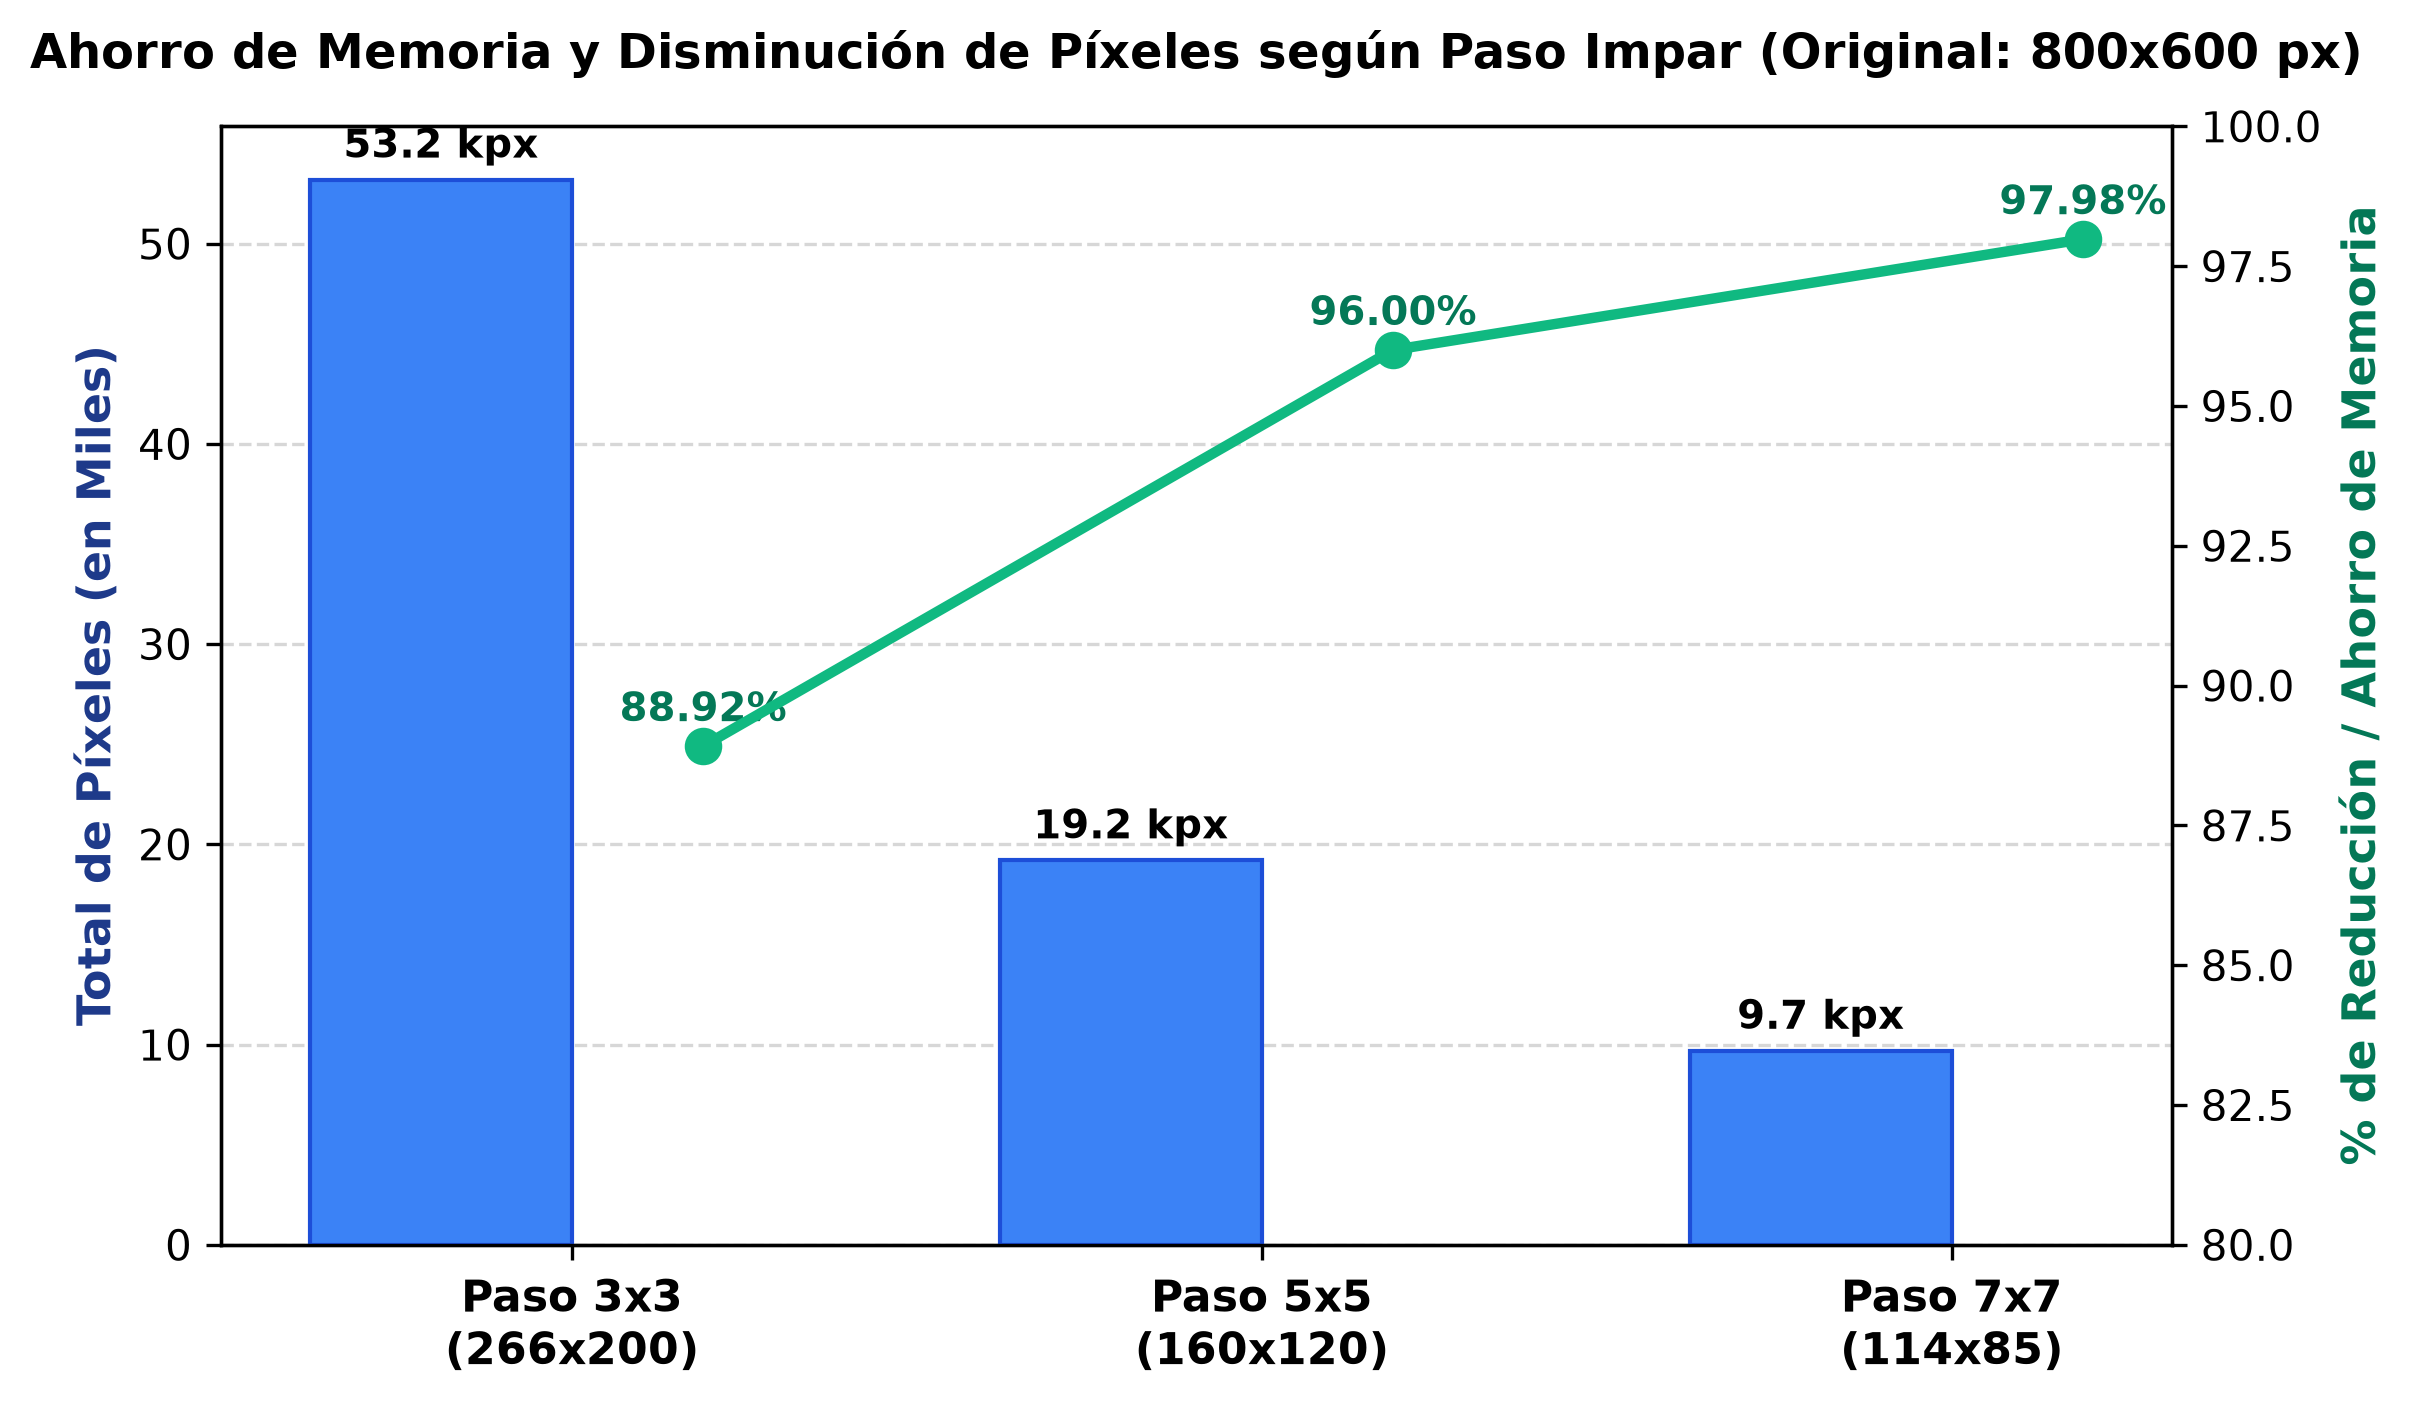
\includegraphics[width=0.82\textwidth]{imagenes/grafico_ahorro_datos.png}
    \caption{Curva de disminución de píxeles totales (en miles) y tasa porcentual de ahorro de datos según el factor de paso impar $k \in \{3, 5, 7\}$.}
    \label{fig:grafico_ahorro}
\end{figure}

\subsection{Demostración Matricial del Mapeo de Píxeles}
La Figura~\ref{fig:matriz_bloque} detalla el proceso físico exacto que experimenta un bloque de $3 \times 3$ píxeles contiguos en la escala de grises. Se aprecia con nitidez cómo los 9 valores de entrada son transformados determinísticamente a un único píxel escalar de salida según el operador seleccionado.

\begin{figure}[H]
    \centering
    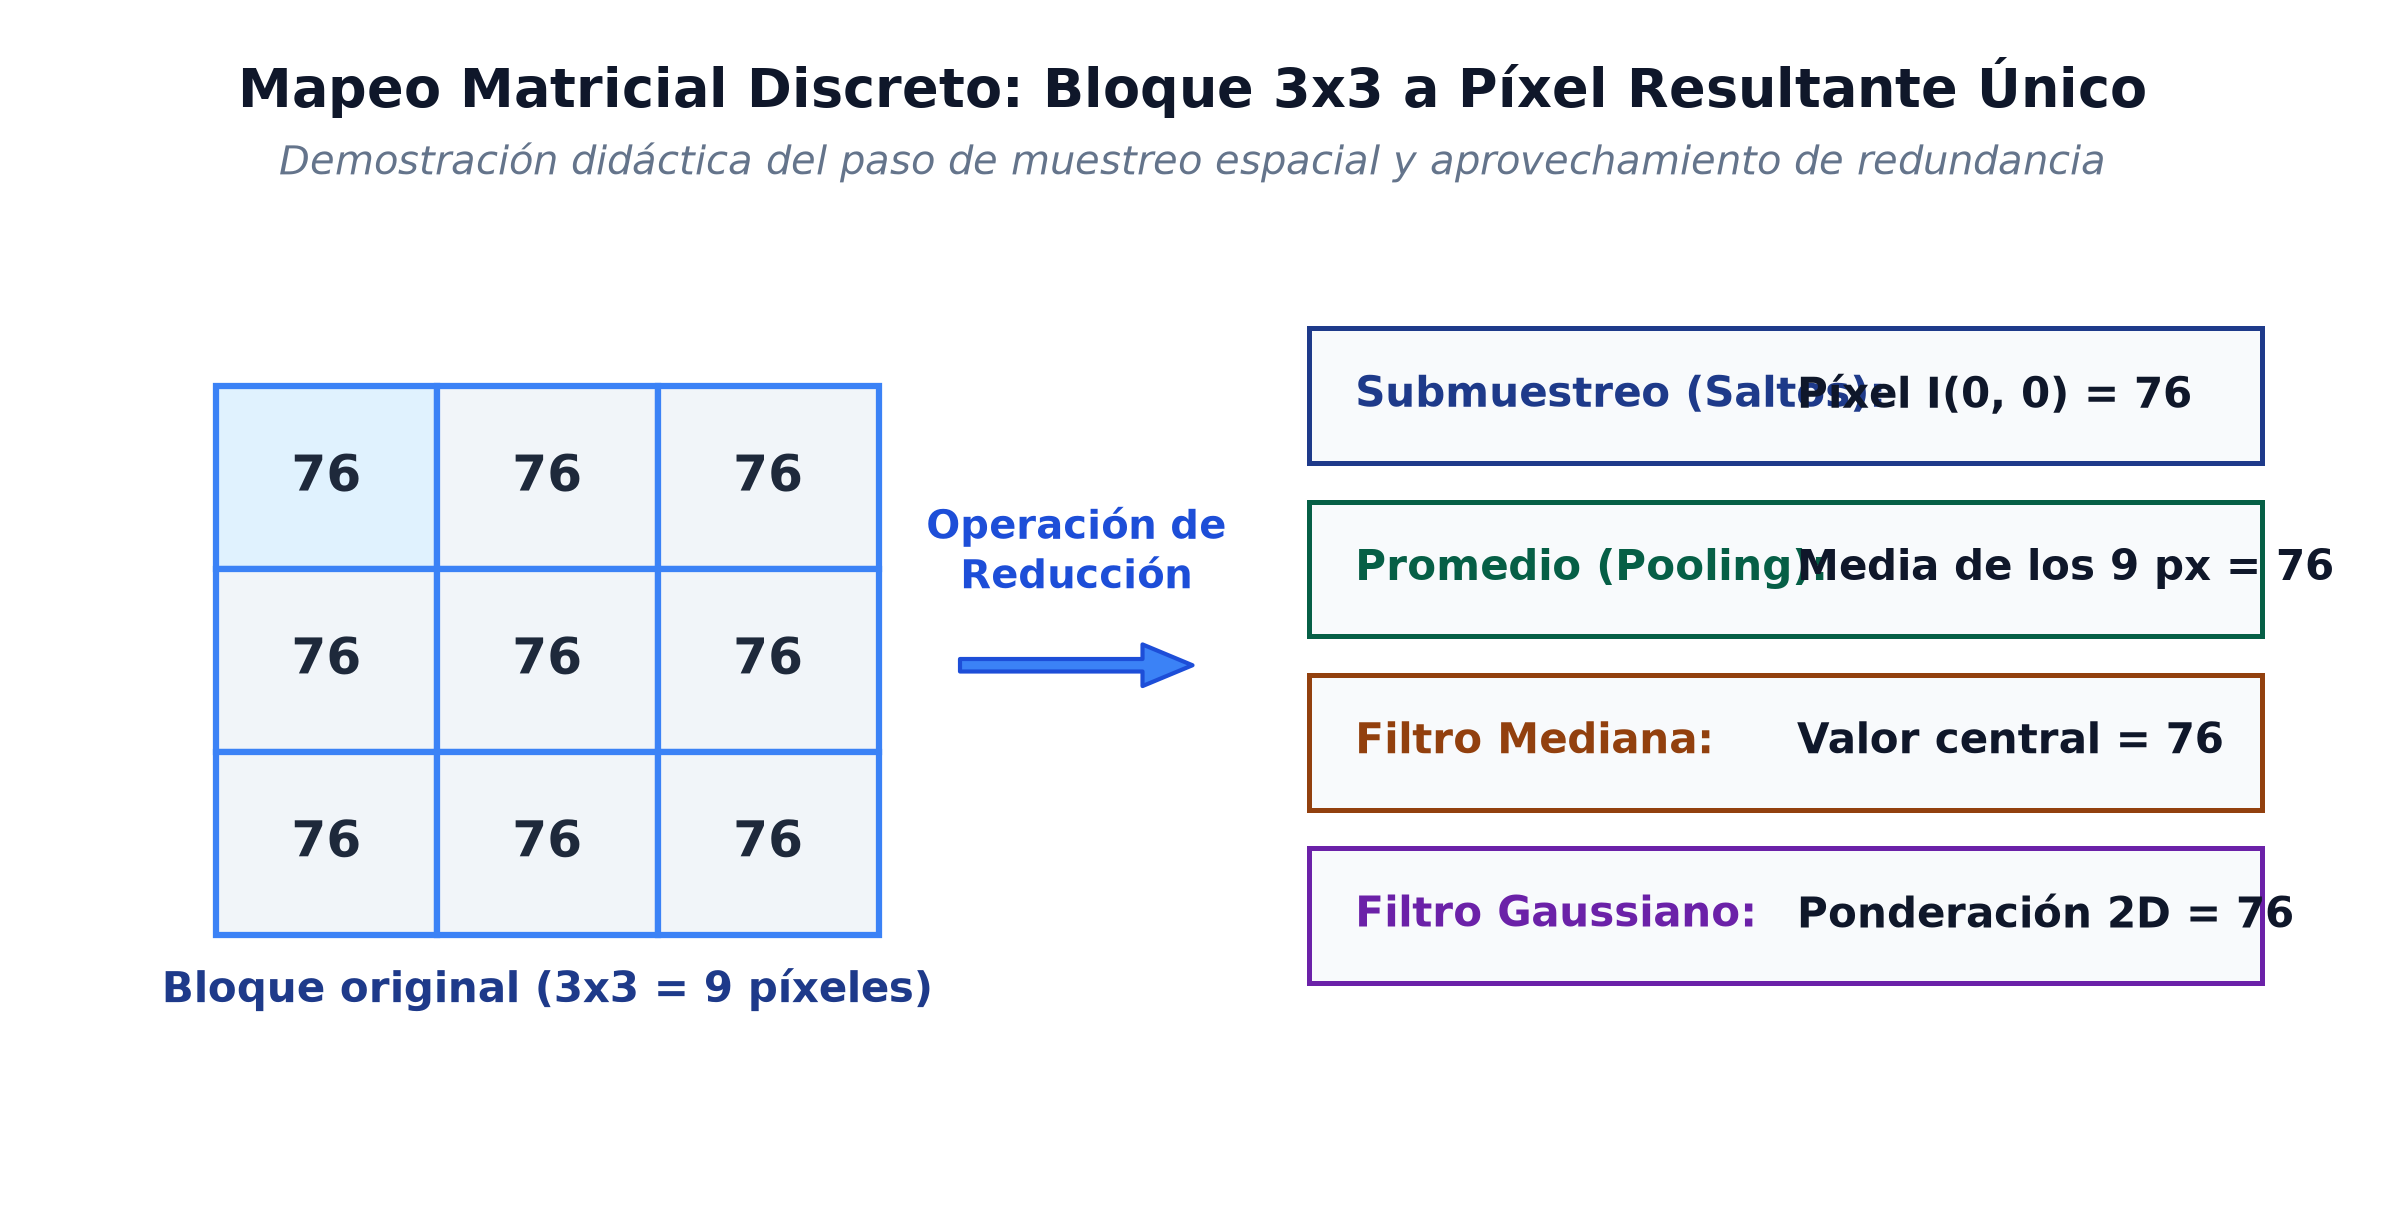
\includegraphics[width=0.92\textwidth]{imagenes/matriz_bloque_explicacion.png}
    \caption{Demostración didáctica del mapeo discreto: bloque de $3\times3$ píxeles originales y valor numérico de salida obtenido por cada uno de los cuatro algoritmos.}
    \label{fig:matriz_bloque}
\end{figure}

\subsection{Análisis Visual Comparativo de los Métodos}
Las Figuras~\ref{fig:comparativa_3} y \ref{fig:comparativa_5} muestran la comparativa visual de los resultados obtenidos para pasos $k = 3$ y $k = 5$ respectivamente.

\begin{figure}[H]
    \centering
    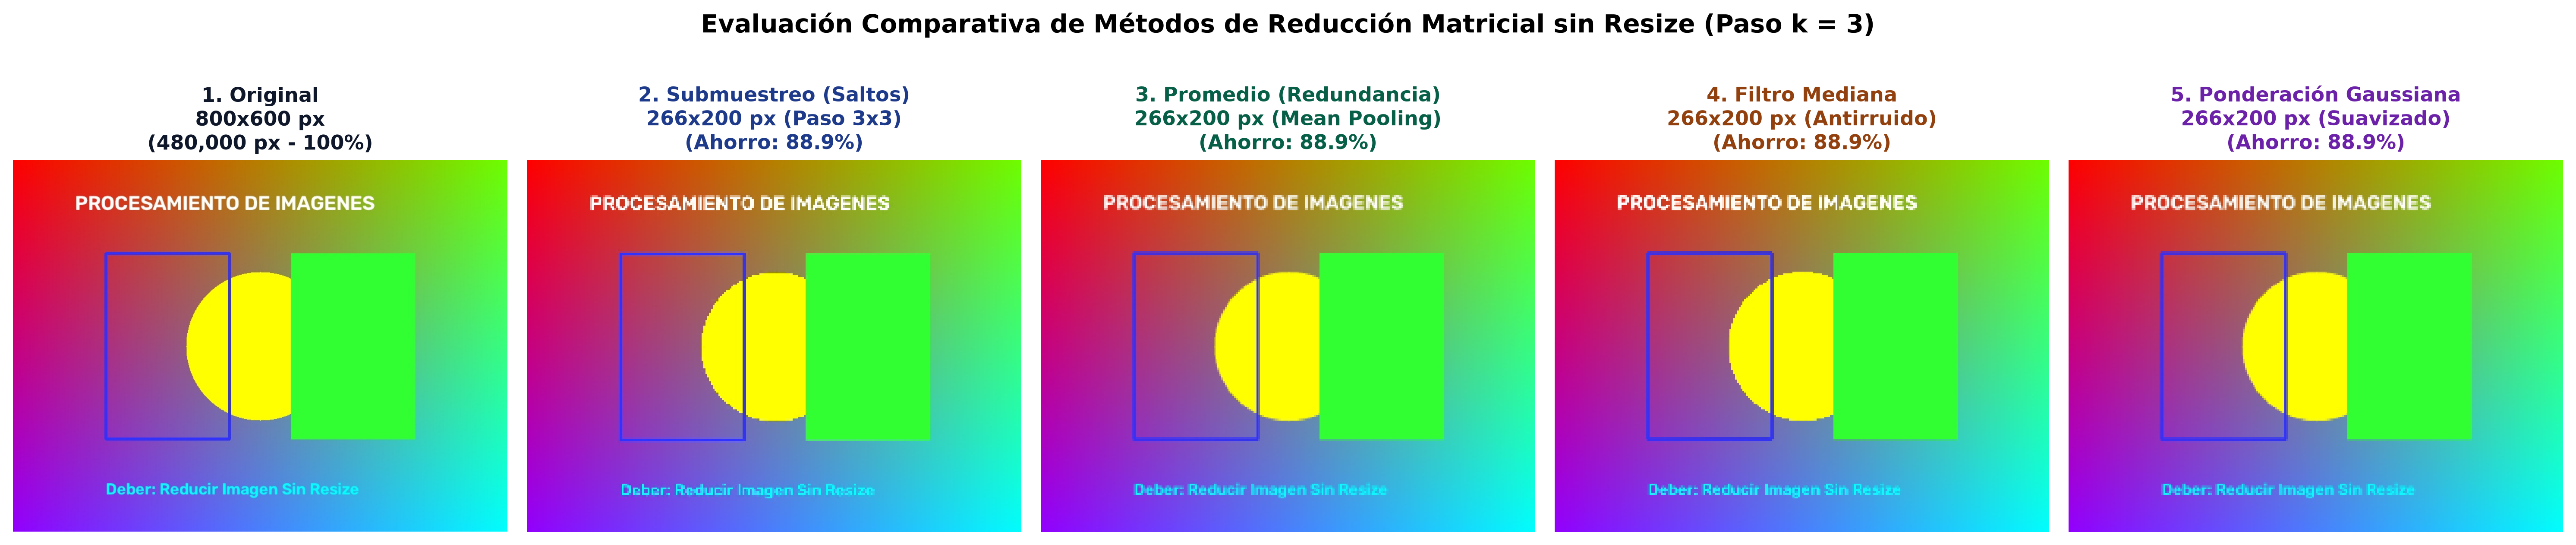
\includegraphics[width=\textwidth]{imagenes/comparativa_paso_3.png}
    \caption{Comparativa visual de los cuatro métodos de reducción para paso impar $k = 3$ (reducción a $266 \times 200$ píxeles, $88.9\%$ de ahorro).}
    \label{fig:comparativa_3}
\end{figure}

\begin{figure}[H]
    \centering
    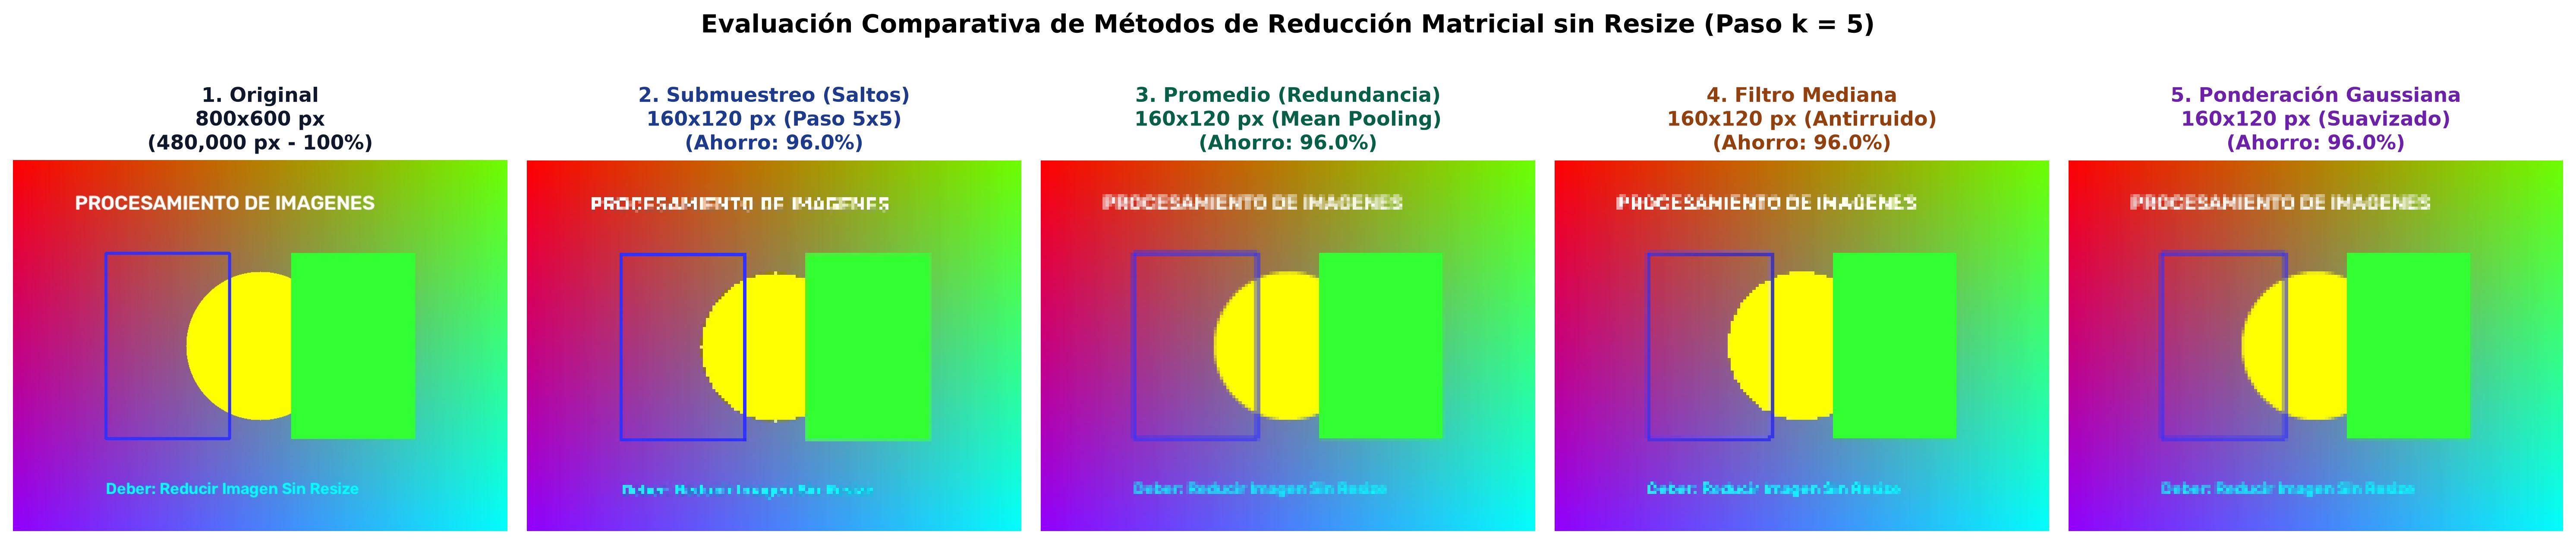
\includegraphics[width=\textwidth]{imagenes/comparativa_paso_5.png}
    \caption{Comparativa visual de los cuatro métodos de reducción para paso impar $k = 5$ (reducción a $160 \times 120$ píxeles, $96.0\%$ de ahorro).}
    \label{fig:comparativa_5}
\end{figure}

Del análisis detallado de las imágenes reducidas se desprenden las siguientes observaciones científicas:
\begin{enumerate}
    \item \textbf{Conservación de la Inteligibilidad:} A pesar de reducir la cantidad de píxeles a tan solo un $11.1\%$ del original en $k=3$ y un $4.0\%$ en $k=5$, todos los métodos preservan plenamente las formas, contornos y contenido de la escena. Esto confirma de manera concluyente la hipótesis de la \textbf{redundancia espacial}: la vecindad inmediata contiene información altamente correlacionada que permite reconocer los objetos con una fracción mínima de muestras.
    \item \textbf{Efecto de Aliasing en el Submuestreo por Saltos:} El método de saltos directos exhibe artefactos visibles de pixelado y bordes serrados en las líneas diagonales y texturas finas. Esto ocurre porque la decimación omite el filtrado de paso bajo previo, violando el criterio de Nyquist.
    \item \textbf{Balance y Suavidad en Promedio y Gaussiana:} Tanto el método de promedio como la convolución gaussiana presentan transiciones tonales notablemente más suaves y naturales. La gaussiana, al concentrar su energía en el centro geométrico, evita la pérdida excesiva de contraste en bordes que a veces aqueja al promedio simple.
    \item \textbf{Estabilidad del Filtro Mediana:} La mediana retiene la nitidez de los bordes estructurales con mayor vigor que el promedio, evitando la borrosidad difusa al tiempo que elimina cualquier ruido impulsivo localizado.
\end{enumerate}

% =========================================================
% 6. BANCO DE PREGUNTAS TÉCNICAS PARA LA SUSTENTACIÓN
% =========================================================

\section{Banco de Preguntas Técnicas para la Sustentación}

Para consolidar la preparación académica y defender los resultados obtenidos ante el docente evaluador, se estructuran las siguientes preguntas conceptuales y técnicas clave:

\begin{description}
    \item[\textbf{Pregunta 1: ¿Por qué el docente prohibió el uso de \texttt{imresize} o \texttt{cv2.resize}?}]~\\
    \textit{Respuesta:} Porque dichas funciones aplican interpolaciones automáticas de caja negra (bilineal, bicúbica o Lanczos) que realizan aproximaciones polinomiales complejas, impidiendo evaluar el objetivo pedagógico del taller: comprender la manipulación directa de índices en matrices bidimensionales y el muestreo espacial discreto.
    
    \item[\textbf{Pregunta 2: Si aplicamos un paso $k = 3$, ¿a cuánto se reduce la cantidad total de píxeles y por qué no a la tercera parte?}]~\\
    \textit{Respuesta:} Se reduce a la \textbf{novena parte} ($\approx 11.11\%$ de los píxeles originales, es decir, un $88.89\%$ de ahorro), debido a que la reducción ocurre simultáneamente en dos dimensiones ortogonales: alto ($1/k$) y ancho ($1/k$), dando como factor de área:
    \begin{equation}
        \text{Factor de escala bidimensional} = \frac{1}{k} \times \frac{1}{k} = \frac{1}{k^2} = \frac{1}{3^2} = \frac{1}{9}
    \end{equation}

    \item[\textbf{Pregunta 3: ¿Cuál es la diferencia matemática fundamental entre el método de saltos y el de promedio?}]~\\
    \textit{Respuesta:} El método de saltos realiza una decimación espacial pura descartando $(k^2 - 1)$ píxeles del bloque sin procesarlos, lo que genera aliasing. El método de promedio calcula una combinación lineal uniforme ponderada por $1/k^2$, actuando como un filtro pasa-bajos que aprovecha la redundancia espacial y preserva la energía luminosa media de la escena.

    \item[\textbf{Pregunta 4: ¿Por qué es matemáticamente obligatorio utilizar matrices de tamaño impar ($3\times3, 5\times5, 7\times7$)?}]~\\
    \textit{Respuesta:} Por tres razones determinantes: 1) Tienen un centro geométrico entero simétrico en $((k-1)/2, (k-1)/2)$; 2) El cardinal $k^2$ es impar, lo que garantiza que la mediana sea un píxel real de la escena sin requerir promedios artificiales; y 3) Permiten construir máscaras gaussianas isotrópicas simétricas alrededor de su centro.

    \item[\textbf{Pregunta 5: ¿Cómo se maneja una imagen a color frente a una en escala de grises?}]~\\
    \textit{Respuesta:} En escala de grises se opera sobre una matriz bidimensional $M \times N$. En color se trabaja sobre un tensor tridimensional $M \times N \times 3$, aplicando el algoritmo de manera desacoplada e idéntica a cada canal cromático (Rojo, Verde y Azul) y recombinándolos posteriormente.
\end{description}

% =========================================================
% 7. CONCLUSIONES Y RECOMENDACIONES
% =========================================================

\section{Conclusiones y Recomendaciones}

\subsection{Conclusiones}
\begin{enumerate}
    \item Se implementaron de forma exitosa los cuatro métodos de reducción dimensional matricial en Python (saltos, promedio, mediana y gaussiana) sin requerir funciones empaquetadas como \texttt{cv2.resize} o \texttt{imresize}, validando la eficacia del cálculo matricial directo mediante \texttt{NumPy}.
    \item Se demostró cuantitativamente que el factor de reducción espacial escala de forma cuadrática ($1/k^2$), logrando reducciones de datos del $88.92\%$ para $k=3$, $96.00\%$ para $k=5$ y $97.98\%$ para $k=7$, lo que evidencia su utilidad crítica para optimizar el preprocesamiento de imágenes en sistemas de inteligencia artificial.
    \item Se justificó analítica y geométricamente la necesidad de emplear bloques de orden impar ($3\times3, 5\times5, 7\times7$), dado que aseguran la existencia de un centro geométrico simétrico entero y posibilitan el cómputo de la mediana pura sin interpolaciones artificiales.
    \item La comparación visual corroboró el principio de redundancia espacial: los píxeles adyacentes presentan una elevada correlación lumínica, lo cual permite que la imagen reducida conserve plenamente su interpretabilidad semántica y estructural.
\end{enumerate}

\subsection{Recomendaciones}
\begin{enumerate}
    \item Para sistemas de visión por computador en tiempo real (como detección de objetos en video con YOLO), se recomienda emplear el método de promedio o gaussiana con $k=3$, ya que equilibra de manera óptima una reducción del $88.9\%$ de datos con una excelente atenuación del ruido y el aliasing.
    \item En presencia de imágenes con sensores ruidosos o artefactos de transmisión de tipo sal y pimienta, se aconseja priorizar el método de mediana por su probada robustez no lineal.
    \item Extender la presente práctica hacia la construcción de pirámides gaussianas y laplacianas multiescala, base fundamental de algoritmos modernos de fusión de imágenes y detección de características como SIFT y SURF.
\end{enumerate}

% =========================================================
% REFERENCIAS BIBLIOGRÁFICAS
% =========================================================

\newpage
\printbibliography[heading=bibintoc, title={Referencias Bibliográficas}]

\end{document}
